\documentclass{beamer}
% all hail op for the og format
\usepackage[english]{babel}
\usepackage{microtype}
\usepackage{enumerate}
% \usepackage{listings}
\usepackage{hyperref}
\usepackage{graphicx}
\usepackage{float}
% \usepackage{amsmath}
\usepackage{blindtext}


\title{Parallel Architecture \& Distributed Architecture (18CS73)}
\author{Atreya Bain (1RV18CS030)\\Chirag Bapat (1RV18CS048)}
\newcommand{\problemtitle}[0]{HDR Tonemapping}

\institute[RVCE]
{
    Submitted To: Dr. Minal Moharir\\
    Associate Professor
    \and
    Self Study Assignment
}
\logo{
\includegraphics[width=0.5cm]{media/rv}}

\begin{document}
% fill in the title stuff
\frame{\maketitle}



\begin{frame}
    \frametitle{Topic}
    \begin{center}
        \LARGE{\problemtitle}
    \end{center}
\end{frame}


\begin{frame}
    \frametitle{Problem Statement}
    Implement HDR Tonemapping to display HDR images, using the Luminance remapping technique on a GPU using CUDA.
\end{frame}


\begin{frame}
    \frametitle{Introduction - Continuation}
    \begin{itemize}
        \item HDR Images contain high precision and high dynamic range image pixel data.
        \item HDR displays can show these by changing the brightness of that section of the screen.
        \item Showing HDR Image on a standard image? Eg. A Sunrise photo
        \begin{itemize}
            \item Linearly scale - Bright parts of the image will make the image mostly dark and unviewable.
            \item Tonemap - Scale the brightness so that the image is still viewable.
        \end{itemize}
    \end{itemize}
\end{frame}

\begin{frame}
    \frametitle{Introduction}
    Tone mapping is a technique used in image processing and computer graphics to map one set of colors to another to approximate the appearance of high-dynamic-range images in a medium that has a more limited dynamic range.
    
    \begin{center}
        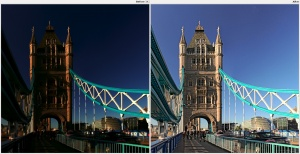
\includegraphics[width=.75\textwidth]{media/300px-Rt407-ba-tonemapping-hdr-cropped.jpg}
        % \caption{Tonemapping - }
    \end{center}
\end{frame}

\begin{frame}
    \frametitle{Methodology}
    \begin{itemize}
        
        \item There are two ways to bring about tonemapping:
        \begin{enumerate}
            \item Global operators: Non-linear functions based on the luminance and other global variables of the image.
            \item Local operators: the parameters of the non-linear function change in each pixel, according to features extracted from the surrounding parameters. Those algorithms are more complicated; they can show artifacts, but they can (if used correctly) provide the best performance, since human vision is mainly sensitive to local contrast.
        \end{enumerate}
    \end{itemize}
    

\end{frame}

\begin{frame}
    \frametitle{Methodology - Luminance Model}
    A good way to begin with
    \begin{itemize}
        \item The YC$_b$C$_r$ color space is a popular color space used in TVs, as it splits out a luminance component (the black and white) and 2 color components.
        \begin{itemize}
            \item Traditionally, the color TVs would use this as a way of displaying color, and the B\&W TVs would simply display only the luminance component, saving on hardware and bandwidth costs.
        \end{itemize} 
        \item The $Y$ component can be scaled here accordingly to change the brightness of that region of the image.
    \end{itemize}
    

\end{frame}

\begin{frame}
    \frametitle{Methodology (Continued)}
            
            \begin{figure}
                \centering
                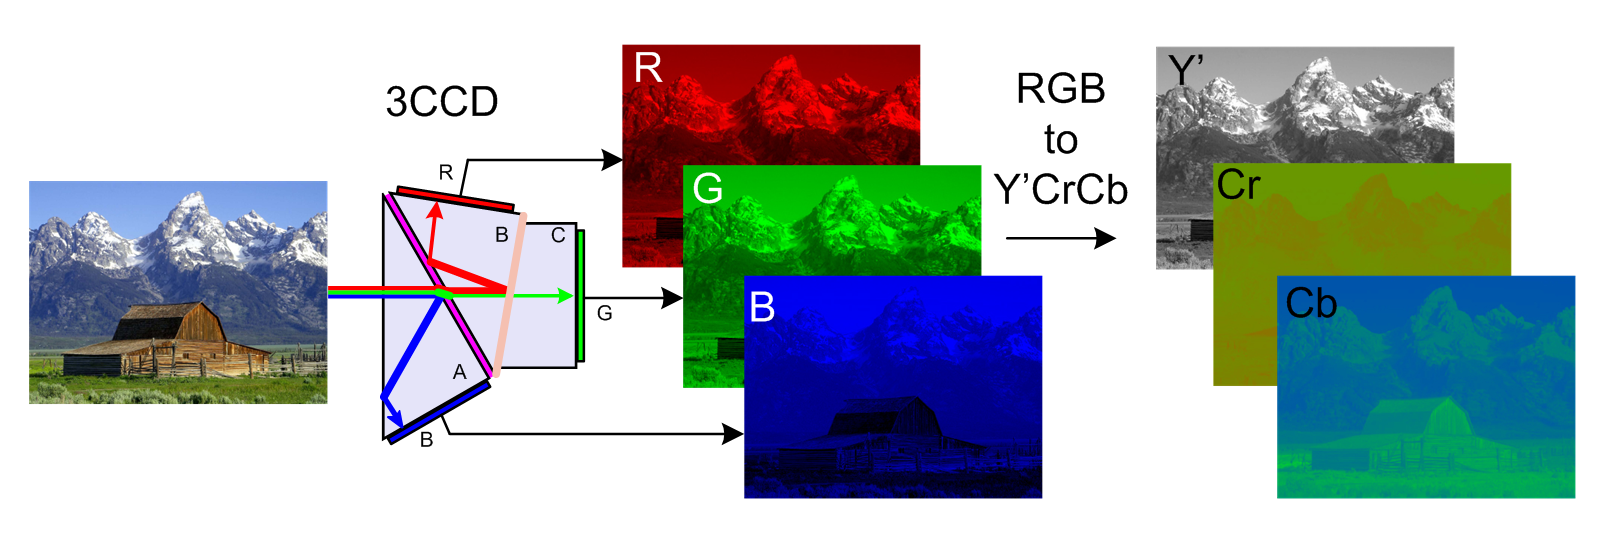
\includegraphics[width=.85\linewidth]{media/CCD.png}
                \caption{RGB to YC$_b$C$_r$}
            \end{figure}

\end{frame}

\begin{frame}
    \frametitle{Methodology}
    Here is the general description of the procedure:
    \begin{enumerate}
        \item Convert the image the the YC$_b$C$_r$ space.
        \item Construct a histogram of brightness values.
        \item Taking the log of the luminance, scale it according to the histogram.
        \item Process and convert back to RGB model as required.
    \end{enumerate}
    

\end{frame}

\begin{frame}
    \frametitle{Why Parallelize?}
    \begin{itemize}
        \item Tone-mapping is done for images, where there are millions of pixels present.
        \item Processing HDR images and videos can become a repetitive and taxing job for the CPU, and this is best offloaded to the GPU.
        \item This is the perfect opportunity for GPU Acceleration.
    \end{itemize}
    
\end{frame}

\begin{frame}
    \frametitle{Results}
    \begin{itemize}
        \item Prefix sum calculation is a bottleneck - This can be done efficiently with the Hillis Steele prefix calculation algorithm.
        \item Serial and parallel implementation can be proven to be similar - Use differences to measure.
        \item 8-10x improvements in performance over naive implementations
    \end{itemize}
\end{frame}

\begin{frame}
    \frametitle{References}
    % use \cite to refer
    \begin{thebibliography}{00}
        \bibitem{compiler-book}{Hunt, R. 2004. "The Reproduction of Colour in Photography, Printing and Television: 6th Edition." John Wiley \& Sons.}
        % \bibitem{cit1}{Citation 1}
    \end{thebibliography}    

\end{frame}


\end{document}